\documentclass[conference]{IEEEtran}
\IEEEoverridecommandlockouts
\usepackage{cite}
\usepackage{amsmath,amssymb}
\usepackage{graphicx}
\usepackage{booktabs}
\usepackage{url}
\usepackage{array}
\usepackage{multirow}
\graphicspath{{figures/}}

\title{Evidence-Linked Clinical Trial Criterion Screening with a Locally Executable Transformer}
\author{\IEEEauthorblockN{Ahmed Laiq}\IEEEauthorblockA{Individual student research project}}

% frozen manifest SHA-256 65924bda7fe02e4ec640029758bb283bf00b72c58fede55cfa697de04cd61f4f
\newcommand{\BaseAccuracy}{0.146}
\newcommand{\AdaptedAccuracy}{0.704}
\newcommand{\BaseMacroF}{0.137}
\newcommand{\AdaptedMacroF}{0.362}
\newcommand{\BaseEvidenceP}{0.091}
\newcommand{\AdaptedEvidenceP}{0.186}
\newcommand{\BaseEvidenceR}{0.926}
\newcommand{\AdaptedEvidenceR}{0.723}
\newcommand{\BaseEvidenceF}{0.165}
\newcommand{\AdaptedEvidenceF}{0.296}
\newcommand{\BaseIncAcc}{0.253}
\newcommand{\BaseIncF}{0.191}
\newcommand{\BaseIncEvidenceF}{0.286}
\newcommand{\AdaptedIncAcc}{0.720}
\newcommand{\AdaptedIncF}{0.382}
\newcommand{\AdaptedIncEvidenceF}{0.485}
\newcommand{\BaseExcAcc}{0.084}
\newcommand{\BaseExcF}{0.050}
\newcommand{\BaseExcEvidenceF}{0.081}
\newcommand{\AdaptedExcAcc}{0.695}
\newcommand{\AdaptedExcF}{0.205}
\newcommand{\AdaptedExcEvidenceF}{0.142}

\begin{document}
\maketitle

\begin{abstract}
This work implements an end-to-end research prototype that predicts TrialGPT criterion-level eligibility labels and cites source sentences from patient descriptions. We fine-tuned a pinned Qwen2.5-1.5B-Instruct checkpoint using LoRA on the prescribed patient-grouped TrialGPT Criterion Annotations training split. The held-out split contains 206 annotations from eight patients and was evaluated once after a checksummed experiment freeze. Relative to the same base checkpoint, the adapted model improved test accuracy from \BaseAccuracy{} to \AdaptedAccuracy{} and macro-F1 from \BaseMacroF{} to \AdaptedMacroF{}. Evidence micro-F1 increased from \BaseEvidenceF{} to \AdaptedEvidenceF{}. The adapted model nevertheless remains weak on minority labels, and its output should not be interpreted as a clinical enrollment decision. We also implement an explicit key/value-cache decoder, tiled online-softmax attention, and greedy speculative decoding with a 0.5B draft model. Manual cache decoding matched the uncached reference in all six adapter-backed cases; speculative output matched in 36/36 cases, but local speculation was slower than cached target decoding. A local browser application exposes criterion results, exact cited text, review flags, exports, and a live attention comparison.
\end{abstract}

\begin{IEEEkeywords}
clinical trial matching, evidence extraction, LoRA, key/value cache, online softmax, speculative decoding
\end{IEEEkeywords}

\section{Introduction}
Screening a patient record against a trial criterion requires more than topical similarity: inclusion and exclusion polarity, missing information, and evidence location all matter. TrialGPT motivates criterion-level decomposition and evidence inspection, but its published results are not comparable to this assignment's patient-grouped split \cite{jin2024trialgpt}. We implement an independently trained, locally executable prototype using the required TrialGPT Criterion Annotations dataset. Our objective is to expose both useful predictions and the operational limits visible in held-out results.

The contribution is a reproducible pipeline with (1) four-way criterion labels and original sentence IDs; (2) a validation-selected LoRA adapter evaluated against the same untouched test rows as its base model; (3) an examined cache-aware greedy loop, online-softmax attention implementation, and target-verified speculative decoder; and (4) a standalone local browser application. This is a criterion-level research result. The aggregate patient-level status is a transparent rule-based aid, not a labeled or validated trial outcome.

\section{Related Work}
TrialGPT decomposes eligibility matching into interpretable criterion-level operations and motivates the source-linked output used here \cite{jin2024trialgpt}. Qwen2 technical documentation describes the decoder family; we pin exact target and draft checkpoint revisions rather than infer properties from a model-family name \cite{qwen2024}. LoRA freezes pretrained weights and learns low-rank updates \cite{hu2021lora}; it reduces trainable parameters but does not eliminate inference activations or guarantee task improvement. FlashAttention and online attention work show how tiling and stable rescaling can reduce intermediate memory traffic, while a Python implementation should not be expected to match a fused kernel \cite{dao2022flash,rabe2022selfattention}. Speculative decoding verifies draft proposals with a target model, preserving target output under appropriate acceptance and cache rules \cite{leviathan2023speculative}. We implement deterministic greedy verification and measure its local cost rather than assuming a published speedup transfers to our hardware.

\section{Materials and Methods}
\subsection{Dataset and protocol}
We use the required TrialGPT Criterion Annotations release pinned to revision \texttt{1cfcafde94a1560a33b4addc1638664fe28fc059}. Patient IDs are sorted and shuffled with NumPy \texttt{default\_rng(42)}; the prescribed 37/8/8 patient split yields 602 prepared training rows, 206 validation rows, and 206 test rows. One known missing-criterion training row (annotation 883) is quarantined under the documented decision. Data audits confirm patient disjointness and exclude model-generated predictions and explanations from inputs. The final test labels were accessed only by the guarded evaluator after the frozen manifest was written.

Each example contains the patient sentences, criterion type, and criterion text. The prompt asks for JSON with a label from the preserved inclusion or exclusion label set and integer source-sentence IDs. Whole leading sentences are retained under the 1024-token input budget; the output cap is 96 tokens. The parser validates allowed labels and IDs; the application resolves citations to exact source text. No evidence is not treated as proof of ineligibility, and a transparent aggregation forces review for uncertain, invalid, contradictory, or truncated outputs.

\subsection{Models and adaptation}
The target is \texttt{Qwen/Qwen2.5-1.5B-Instruct}, revision \texttt{989aa7980e4cf806f80c7fef2b1adb7bc71aa306}, with the Qwen2 causal decoder and pinned tokenizer. The smaller speculative draft is \texttt{Qwen/Qwen2.5-0.5B-Instruct}, revision \texttt{7ae557604adf67be50417f59c2c2f167def9a775}; vocabulary equality was checked. Both checkpoints use Apache-2.0 model licenses. LoRA targets query and value projections with rank 8, alpha 16, and dropout 0.05. Training uses AdamW at $2\times10^{-4}$, microbatch 1, gradient accumulation 8, gradient checkpointing, FP16, and three epochs. The full run completed 228 optimizer steps on a Colab Tesla T4. Epoch 3 was selected using validation macro-F1 with evidence F1 and validation loss tie-breaks. The adapter was verified locally on an RTX 3050 Laptop GPU with 6 GiB.

\subsection{Decoding and attention}
The canonical generation contract is deterministic greedy decoding with one beam, pinned EOS/pad IDs, and the target generation-config repetition penalty. The uncached reference calls \texttt{generate(use\_cache=False)} so processors remain active. The explicit decoder prefills once, then forwards one committed token at a time with absolute cache positions, a growing attention mask, and cache-length assertions. The speculative path drafts up to $k$ tokens, verifies the block with target logits, accepts the matching prefix, appends the target correction token at the first mismatch, and crops both caches to the committed length. Qwen's history-dependent repetition penalty is applied to both draft and target token histories.

For attention, the dense reference computes scaled dot products in FP32 and handles boolean visibility masks and fully masked rows. The tiled implementation processes query and key blocks while maintaining the online maximum, normalizer, and weighted-value accumulator. It avoids materializing the full score matrix, but its Python loops incur overhead. For a score tile with row maximum $m_t$, normalizer $\ell_t$, and weighted sum $o_t$, a new tile with maximum $m$ is merged using $m\prime=\max(m_t,m)$, $\ell\prime=e^{m_t-m\prime}\ell_t+\sum_j e^{s_j-m\prime}$, and $o\prime=e^{m_t-m\prime}o_t+\sum_j e^{s_j-m\prime}v_j$; the final output is $o/\ell$.

\begin{figure}[t]
\centering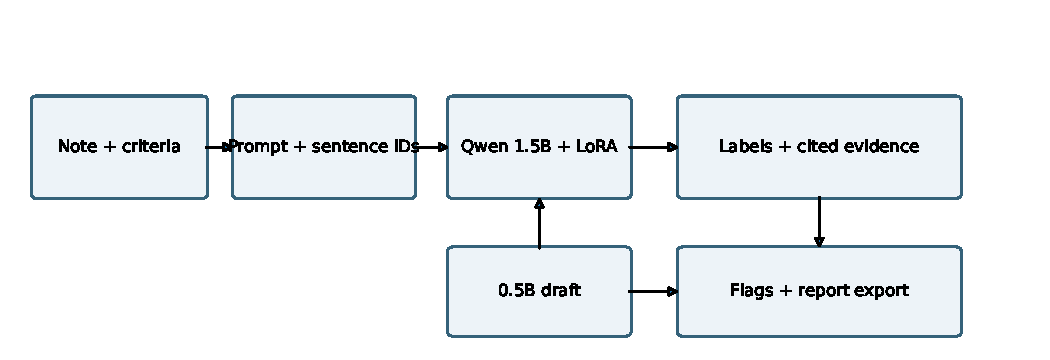
\includegraphics[width=\columnwidth]{system_architecture.pdf}
\caption{End-to-end data flow. The final application loads one adapted target; speculative mode additionally loads the pinned draft. Exact cited sentences and review flags remain visible.}
\label{fig:architecture}
\end{figure}

\section{Experimental Setup and Metrics}
Classification uses accuracy, fixed-class macro-F1, per-class precision/recall/F1, and confusion matrices, overall and by criterion type. Evidence uses micro precision, recall, and F1 over sentence-ID sets; empty gold evidence contributes no true positives and predicted IDs remain false positives. We report overall and inclusion/exclusion results. Tests use the same frozen IDs, prompt, parsing, metric, and generation contract for base and adapted variants.

Local measurements use an RTX 3050 Laptop GPU, CUDA-enabled PyTorch 2.11.0, Transformers 4.57.1, and FP16. Training ran separately on a Colab Tesla T4. Decoder correctness compares token IDs exactly. Timings are local and should not be compared across these hardware environments. The attention experiment uses synthetic tensors and does not claim a transformer-kernel speedup.

\section{Results}
\subsection{Held-out criterion performance}
Table~\ref{tab:overall} reports the paired final test results. Fine-tuning raises accuracy and macro-F1 while leaving substantial error, particularly among minority labels. The model collapses much of the exclusion task to ``not excluded''; this explains why accuracy alone would give an incomplete view. Evidence recall is higher than evidence precision, reflecting overinclusive citations. The app displays exact cited text and never presents an aggregate preliminary match as ground truth.

\begin{table}[t]
\caption{Final test results on the frozen 206-row split}
\label{tab:overall}
\centering\small
\begin{tabular}{llrr}
\toprule
Task & Metric & Base & Adapted\\
\midrule
Classification & Accuracy & \BaseAccuracy{} & \AdaptedAccuracy{}\\
 & Macro-F1 & \BaseMacroF{} & \AdaptedMacroF{}\\
Evidence & Micro precision & \BaseEvidenceP{} & \AdaptedEvidenceP{}\\
 & Micro recall & \BaseEvidenceR{} & \AdaptedEvidenceR{}\\
 & Micro-F1 & \BaseEvidenceF{} & \AdaptedEvidenceF{}\\
\bottomrule
\end{tabular}
\end{table}

\subsection{Per-type results and errors}
Inclusion and exclusion results are separated in Table~\ref{tab:types}. We provide confusion matrices and a case-level ledger in the generated evidence package. Eight representative errors use eight distinct test patients. Examples include an incorrect ``not enough information'' response to explicit shock-related evidence and an unsupported ``not excluded'' response for criteria with no supporting source. The error ledger preserves the gold/predicted evidence excerpts and raw structured output. These examples demonstrate category confusion and evidence overreach; they do not establish why the model produced an answer.

\begin{table}[t]
\caption{Test metrics by criterion type}
\label{tab:types}
\centering\small
\begin{tabular}{llrr}
\toprule
Type & Metric & Base & Adapted\\
\midrule
Inclusion & Accuracy & \BaseIncAcc{} & \AdaptedIncAcc{}\\
 & Macro-F1 & \BaseIncF{} & \AdaptedIncF{}\\
 & Evidence micro-F1 & \BaseIncEvidenceF{} & \AdaptedIncEvidenceF{}\\
Exclusion & Accuracy & \BaseExcAcc{} & \AdaptedExcAcc{}\\
 & Macro-F1 & \BaseExcF{} & \AdaptedExcF{}\\
 & Evidence micro-F1 & \BaseExcEvidenceF{} & \AdaptedExcEvidenceF{}\\
\bottomrule
\end{tabular}
\end{table}

\begin{table*}[t]\centering\caption{Per-class test precision, recall, F1, and support.}\small\begin{tabular}{lllrrrr}\toprule Type & Variant & Class & Precision & Recall & F1 & Support \\
\midrule
Inclusion & Base & included & 0.73 & 0.59 & 0.65 & 27 \\
Inclusion & Base & not applicable & 0.06 & 1.00 & 0.11 & 3 \\
Inclusion & Base & not enough information & 0.00 & 0.00 & 0.00 & 38 \\
Inclusion & Base & not included & 0.00 & 0.00 & 0.00 & 7 \\
Inclusion & Adapted & included & 1.00 & 0.59 & 0.74 & 27 \\
Inclusion & Adapted & not applicable & 0.00 & 0.00 & 0.00 & 3 \\
Inclusion & Adapted & not enough information & 0.64 & 1.00 & 0.78 & 38 \\
Inclusion & Adapted & not included & 0.00 & 0.00 & 0.00 & 7 \\
Exclusion & Base & excluded & 0.00 & 0.00 & 0.00 & 0 \\
Exclusion & Base & not applicable & 0.11 & 0.92 & 0.20 & 12 \\
Exclusion & Base & not enough information & 0.00 & 0.00 & 0.00 & 28 \\
Exclusion & Base & not excluded & 0.00 & 0.00 & 0.00 & 91 \\
Exclusion & Adapted & excluded & 0.00 & 0.00 & 0.00 & 0 \\
Exclusion & Adapted & not applicable & 0.00 & 0.00 & 0.00 & 12 \\
Exclusion & Adapted & not enough information & 0.00 & 0.00 & 0.00 & 28 \\
Exclusion & Adapted & not excluded & 0.69 & 1.00 & 0.82 & 91 \\
\bottomrule\end{tabular}\end{table*}
\begin{table*}[t]\centering\caption{Test confusion matrices by criterion type and model variant. Rows are gold; columns are predicted.}\scriptsize\begin{tabular}{lrrrrrr}\toprule
\multicolumn{7}{l}{Inclusion / Base} \\
Gold / Pred. & included & not included & not enough information & not applicable & \_\_invalid\_\_ & Support \\
\midrule
included & 16 & 0 & 0 & 11 & 0 & 27 \\
not included & 3 & 0 & 0 & 4 & 0 & 7 \\
not enough information & 3 & 0 & 0 & 34 & 1 & 38 \\
not applicable & 0 & 0 & 0 & 3 & 0 & 3 \\
\_\_invalid\_\_ & 0 & 0 & 0 & 0 & 0 & 0 \\
\multicolumn{7}{l}{Inclusion / Adapted} \\
Gold / Pred. & included & not included & not enough information & not applicable & \_\_invalid\_\_ & Support \\
\midrule
included & 16 & 0 & 11 & 0 & 0 & 27 \\
not included & 0 & 0 & 7 & 0 & 0 & 7 \\
not enough information & 0 & 0 & 38 & 0 & 0 & 38 \\
not applicable & 0 & 0 & 3 & 0 & 0 & 3 \\
\_\_invalid\_\_ & 0 & 0 & 0 & 0 & 0 & 0 \\
\multicolumn{7}{l}{Exclusion / Base} \\
Gold / Pred. & excluded & not excluded & not enough information & not applicable & \_\_invalid\_\_ & Support \\
\midrule
excluded & 0 & 0 & 0 & 0 & 0 & 0 \\
not excluded & 27 & 0 & 0 & 64 & 0 & 91 \\
not enough information & 6 & 0 & 0 & 22 & 0 & 28 \\
not applicable & 1 & 0 & 0 & 11 & 0 & 12 \\
\_\_invalid\_\_ & 0 & 0 & 0 & 0 & 0 & 0 \\
\multicolumn{7}{l}{Exclusion / Adapted} \\
Gold / Pred. & excluded & not excluded & not enough information & not applicable & \_\_invalid\_\_ & Support \\
\midrule
excluded & 0 & 0 & 0 & 0 & 0 & 0 \\
not excluded & 0 & 91 & 0 & 0 & 0 & 91 \\
not enough information & 0 & 28 & 0 & 0 & 0 & 28 \\
not applicable & 0 & 12 & 0 & 0 & 0 & 12 \\
\_\_invalid\_\_ & 0 & 0 & 0 & 0 & 0 & 0 \\
\bottomrule\end{tabular}\end{table*}
\begin{table*}[t]\centering\caption{Eight representative label errors from eight distinct held-out patients. Evidence excerpts are exact source spans, shortened only at display boundary.}
\scriptsize\setlength{\tabcolsep}{2pt}\begin{tabular}{p{1.6cm}p{3.5cm}p{2.5cm}p{4.5cm}p{4.5cm}}\toprule Annotation / type & Criterion & Gold to predicted & Gold evidence excerpt & Predicted evidence excerpt \\
\midrule
161 / Inclusion & Patients undergoing elective carotid endarterectomy & not included $\rightarrow$ not enough information & (no cited sentence IDs) & A physician is called to see a 67-year-old woman... \\
185 / Inclusion & Patients were included if they were diagnosed with Shock, ... & included $\rightarrow$ not enough information & On examination she is pale and in moderate disco... & A 40-year-old woman with no past medical history... \\
315 / Exclusion & BMI> 40 kg/m2. & not enough information $\rightarrow$ not excluded & (no cited sentence IDs) & A 48-year-old white male with history of common ... \\
382 / Inclusion & Fulfil at least 4 criteria for SLE as defined by the Ameri... & included $\rightarrow$ not enough information & A 21-year-old female is evaluated for progressiv... & A 21-year-old female is evaluated for progressiv... \\
418 / Exclusion & Failure to pass MRI metal screening & not enough information $\rightarrow$ not excluded & (no cited sentence IDs) & On an abdominal ultrasound, a markedly edematous... \\
682 / Inclusion & Primary indication for AT is nocturnal obstructive symptom... & included $\rightarrow$ not enough information & A 10 yo boy with nighttime snoring, pauses in br... & A 10 yo boy with nighttime snoring, pauses in br... \\
745 / Inclusion & female patients have adequate birth-control method & not applicable $\rightarrow$ not enough information & (no cited sentence IDs) & A 5-year-old boy presents to the emergency depar... \\
834 / Inclusion & --Negative pregnancy test for females & not applicable $\rightarrow$ not enough information & (no cited sentence IDs) & A 4 year old boy presents to the emergency room ... \\
\bottomrule\end{tabular}\end{table*}
\subsection{Inference mechanisms}
The adapter-backed explicit cache path matches the uncached reference in 6/6 validation cases over three prompt lengths and two output caps. The adapter-backed speculative target matched exactly in 36/36 validation cases over three prompts, caps 8/16/32, and $k=1/2/4/8$. On one 356-token validation prompt with a 16-token cap, ordinary cached target generation took 0.930 s median. Speculative $k=2$ took 1.402 s (0.664$\times$ speedup, i.e., slower); $k=8$ took 2.167 s (0.429$\times$). The 0.5B draft was resident alongside the 1.5B target, with peak allocated memory around 4.22--4.34 GB. Correctness is established for this sample; a local speedup is not.

For the base target, explicit KV reuse was 2.6--3.0$\times$ faster than the uncached reference on the saved local prompts. With the selected adapter, explicit caching was 2.19$\times$ and 2.94$\times$ faster on 335- and 356-token validation prompts, respectively, at a 16-token cap (five repetitions per mode). The attention benchmark compared dense and tiled methods across sequence lengths 128--2048 and tile widths 16/32/64, with five synchronized repetitions. Numerical errors remained small, but the simple tiled implementation was slower because Python launches and loop overhead dominate. Figure~\ref{fig:training} summarizes adapter training loss; Figure~\ref{fig:performance} compares the final test metrics.

\begin{figure}[t]
\centering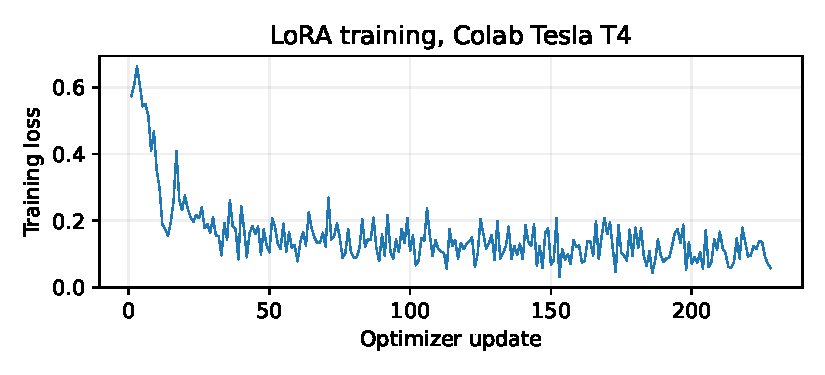
\includegraphics[width=\columnwidth]{training_loss.pdf}
\caption{Training loss across 228 optimizer updates. Validation selected epoch 3; this curve is not a test-set tuning signal.}
\label{fig:training}
\end{figure}
\begin{figure}[t]
\centering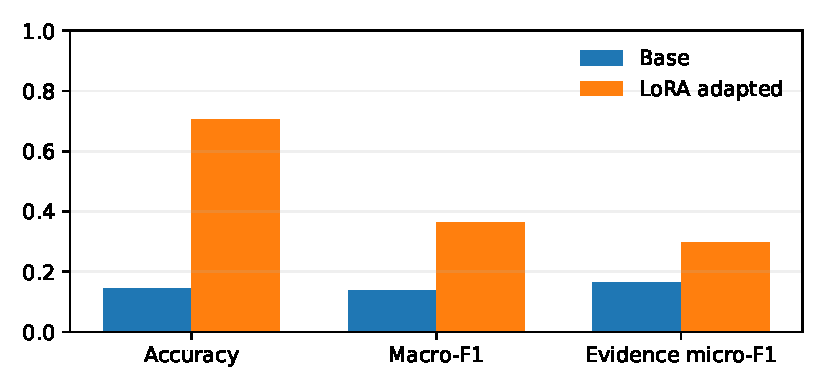
\includegraphics[width=\columnwidth]{test_metrics.pdf}
\caption{Paired held-out accuracy, macro-F1, and evidence micro-F1. Fine-tuning improves all three aggregate measures on the frozen split.}
\label{fig:performance}
\end{figure}

\begin{figure}[t]
\centering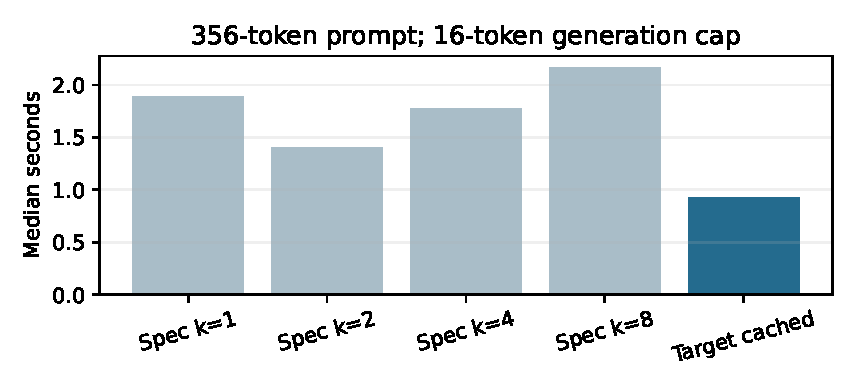
\includegraphics[width=\columnwidth]{decoder_benchmarks.pdf}
\caption{Adapter-backed speculative decoding latency versus cached target greedy decoding on one validation prompt. Lower is faster; target-only is the reference.}
\label{fig:decoderbench}
\end{figure}
\begin{figure}[t]
\centering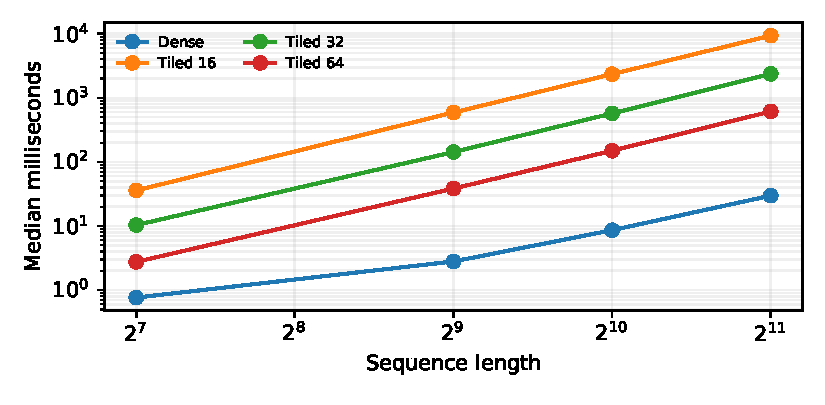
\includegraphics[width=\columnwidth]{attention_runtime.pdf}
\caption{Dense and tiled online-softmax attention median latency on the RTX 3050 Laptop GPU. Five timed repetitions per setting; values are not transformer inference timings.}
\label{fig:attentionbench}
\end{figure}

\begin{figure}[t]
\centering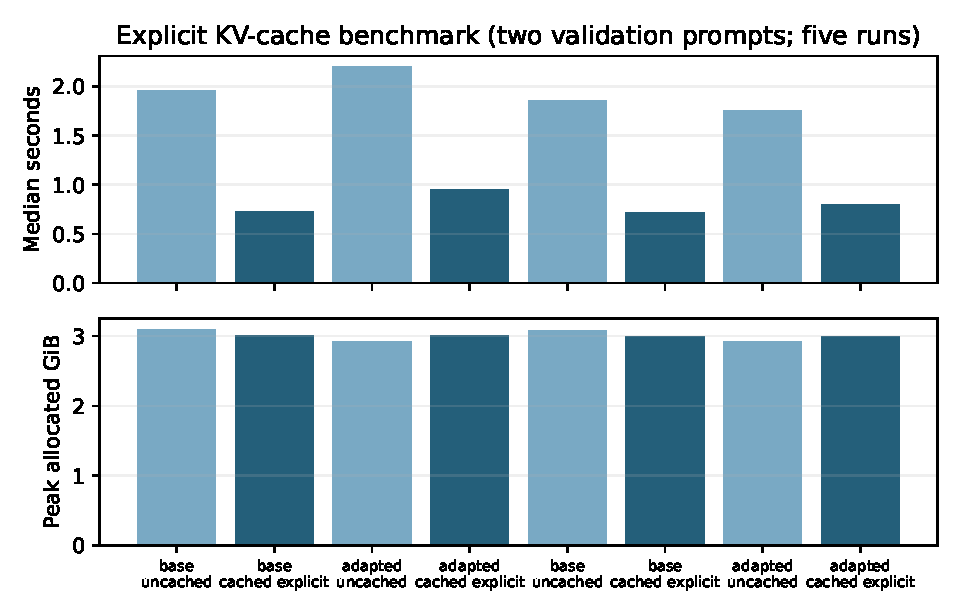
\includegraphics[width=\columnwidth]{cache_benchmarks.pdf}
\caption{Adapted cache path versus uncached generation on two validation prompts. Bars show median latency and peak allocated memory over five repetitions on the local RTX 3050.}
\label{fig:cachebench}
\end{figure}
\begin{figure}[t]
\centering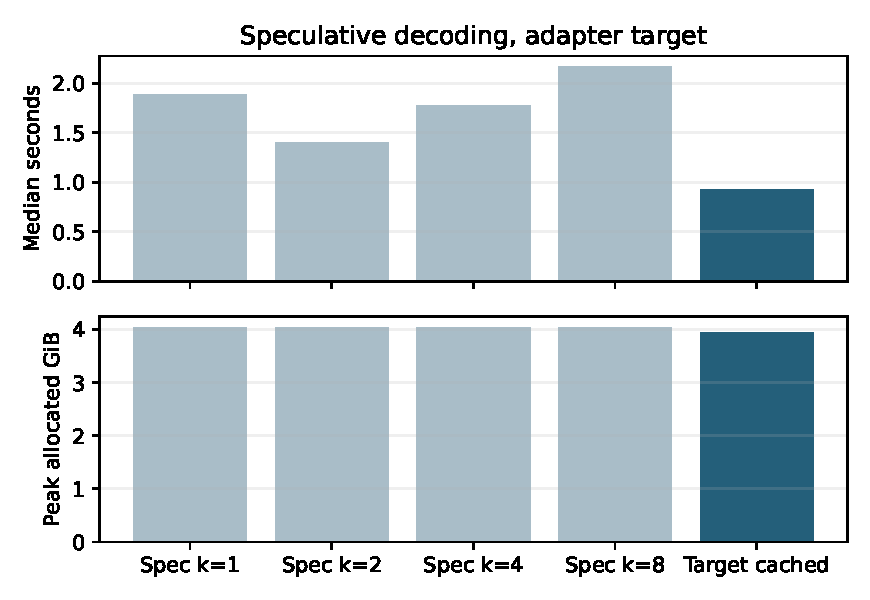
\includegraphics[width=\columnwidth]{speculative_memory.pdf}
\caption{Adapter-backed speculative latency and peak memory with the target and draft resident. Five repetitions on one validation prompt; correctness was exact for every measured mode.}
\label{fig:specmemory}
\end{figure}
\begin{figure}[t]
\centering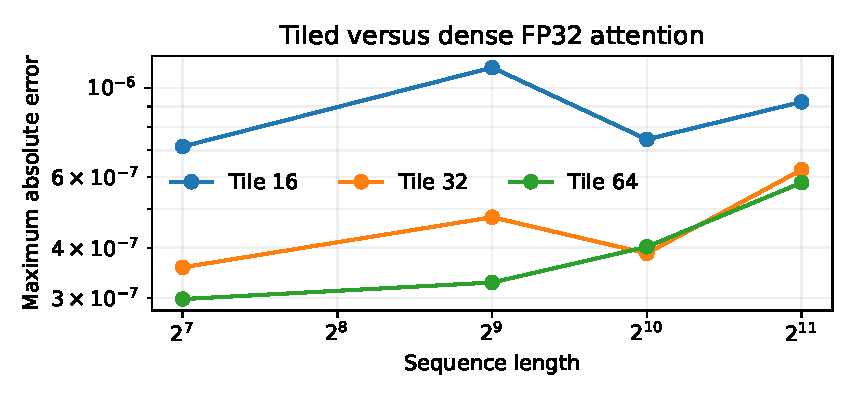
\includegraphics[width=\columnwidth]{attention_error.pdf}
\caption{Maximum absolute output error for tiled online-softmax attention against the dense reference across sequence lengths and tile widths.}
\label{fig:attnerror}
\end{figure}
\begin{figure*}[t]
\centering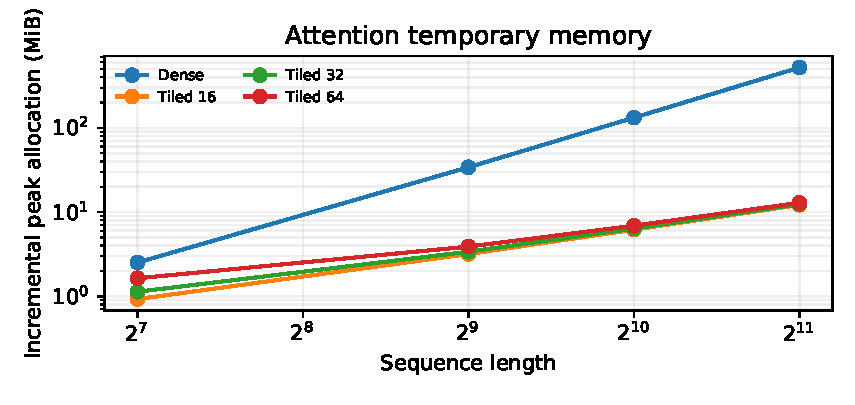
\includegraphics[width=\textwidth]{attention_memory.pdf}
\caption{Incremental peak allocation for the dense and tiled attention routines. At length 2,048, tile width 64 reduced measured incremental peak allocation from approximately 520 MiB to 13 MiB.}
\label{fig:attnmemory}
\end{figure*}

\section{Limitations and Discussion}
The benchmark has 206 criterion annotations from only eight test patients. Label supports are imbalanced, and the adapted model has zero test support for some classes it fails to predict. The results are not clinical validation, external replication, or a trial-level eligibility assessment. Evidence matching is sentence-level set overlap; it does not prove entailment, temporal interpretation, or causal reasoning. The local speculative benchmark uses one prompt and five repetitions, so it supports a hardware-specific slowdown observation rather than a general efficiency claim. The tiled attention kernel is educational Python code, not fused production attention. Colab and laptop results are reported separately. The app is local and offline-capable once model weights and dependencies are present; speculative mode needs additional memory.

\section{Conclusion}
We completed LoRA adaptation and an adapter-backed local screening application, then evaluated base and adapted models once on the same frozen test annotations. Fine-tuning substantially improved aggregate criterion metrics, while severe minority-class and evidence-localization errors remain. The cache-aware decoder, online-softmax attention, and greedy speculative implementation are inspectable and supported by correctness and timing artifacts. The application exposes source-linked predictions, uncertainty, runtime modes, and downloadable reports with a clear educational notice. These results support a demonstration of the implemented system, not clinical use.

\section*{AI-Use Appendix}
AI assistants were used to help plan implementation, draft and revise code/documentation, and review work. The author ran the experiments, inspected the repository and outputs, and is responsible for verifying, explaining, and defending the submitted work. No assistant-generated prediction or explanation was included as a model input feature.

\bibliographystyle{IEEEtran}
\bibliography{references}
\end{document}

